\documentclass[a4paper,12pt]{article}

\usepackage[T1]{fontenc}
\usepackage[utf8]{inputenc}
\usepackage{mortenmath}
\usepackage{amssymb}
\usepackage{commath}
\usepackage{graphicx}
\usepackage{amsmath}
\usepackage{libertine}
\usepackage[hidelinks]{hyperref}

% Make ligatures and stuff copiable from pdf:
\input{glyphtounicode}
\pdfgentounicode=1

\title{Summary of TTK4215:\\System Identification and Adaptive Control}
\author{Morten Fyhn Amundsen \& Erik Liland}
\date{\today}

\begin{document}

\maketitle
\tableofcontents

\section{Todo}
\begin{itemize}
	\item Canoncal forms
	\item Unbounded input (necessary shit for proofs or whatever)
	\item PE (p177)
	\item APPC (brief how-to)
	\item MRAC (brief how-to)
	\item Richness of input and number of parameters.
\end{itemize}

%!TEX root = ../TTK18-Summary.tex
\section{Preliminaries}

% \subsection{KKT conditions}
% Yada yada yada.

\subsection{Lyapunov stability}

\paragraph{Continuous systems}
If there exists a $P > 0$ satisfying
\begin{equation}
  A\tp P + PA < 0,
\end{equation}
then the system $\dot{x} = Ax$ is globally asymptotically stable.

\paragraph{Discrete-time systems}
If there exists a $P > 0$ satisfying
\begin{equation}
  A\tp P A - P < 0,
\end{equation}
then the system $x_{k+1} = Ax_k$ is globally asymptotically stable.

%!TEX root = TTK4215-Summary.tex
\section{Parametric models}

\subsection{Linear}
\begin{equation}
	z = \theta^{*\T} \phi
\end{equation}

\begin{equation}
	y = \theta_\lambda^{*\T} \phi
\end{equation}

\subsection{Bilinear}
\begin{equation}
	y = k_0 (\theta^{*\T} \phi + z_0)
\end{equation}
%!TEX root = TTK4215-Summary.tex
\section{Parameter estimation}

\subsection{SPR Lyapunov method}
Based on choosing an adaptive law so that a \emph{Lyapunov-like} function guarantees $\tilde{\theta} \rightarrow 0$. The parametric model $z = W(s) \theta^{*\T} \psi$ is rewritten $z = W(s) L(s) \theta^{*\T} \phi$, with $L(s)$ a proper stable t.f., and $W(s)L(s)$ a proper SPR t.f.

\begin{gather}
	z = W(s) L(s) \theta^{*\T} \phi \\
	\hat{z} = W(s)L(s) \theta\T \phi \\
	\epsilon = z - \hat{z} - W(s) L(s) \epsilon n_s^2 \\
	\dot{\theta} = \Gamma \epsilon \phi
\end{gather}

\subsection{Gradient method}
\begin{gather}
	z = \theta^{*\T} \phi \\
	\hat{z} = \theta\T \phi \\
	\epsilon = \frac{z - \hat{z}}{m^2}
\end{gather}

\subsubsection{Instantaneous cost}
\begin{gather}
	\dot{\theta} = \Gamma \epsilon \phi
\end{gather}

\subsubsection{Integral cost}
\begin{gather}
	\dot{\theta} = - \Gamma (R \theta + Q) \\
	\dot{R} = - \beta R + \frac{\phi \phi\T}{m^2} \\
	\dot{Q} = - \beta Q - \frac{z \phi}{m^2}
\end{gather}

\subsection{With projection}
\begin{gather}
	\dot{\theta} =
	\begin{cases}
		\Gamma \epsilon \phi & \mbox{if } \theta \in \mathcal{S}^0 \\
		\Gamma \epsilon \phi - \Gamma \frac{\nabla g \nabla g\T}{\nabla g\T \Gamma \nabla g} \Gamma \epsilon \phi & \mbox{otherwise}
	\end{cases}
\end{gather}

\subsection{Least squares}
\begin{gather}
	z = \theta^{*\T} \phi \\
	\hat{z} = \theta\T \phi \\
	\epsilon = \frac{z - \hat{z}}{m^2}
\end{gather}

\subsubsection{Pure least squares}
\begin{gather}
	\dot{\theta} = P \epsilon \phi \\
	\dot{P} = - P \frac{\phi \phi\T}{m^2} P
\end{gather}

\subsubsection{With covariance resetting}
\begin{gather}
	\dot{\theta} = P \epsilon \phi \\
	\dot{P} = - P \frac{\phi \phi\T}{m^2} P, \quad P(t_r^+) = P_0 = \rho_0 I
\end{gather}

\subsubsection{With forgetting}
\begin{gather}
	\dot{\theta} = P \epsilon \phi \\
	\dot{P} =
	\begin{cases}
		\beta P - P \frac{\phi \phi\T}{m^2} P & \mbox{if } ||P(t)|| \leq R_0 \\
		0                                     & \mbox{otherwise}
	\end{cases}
\end{gather}
%!TEX root = TTK4215-Summary.tex
\section{Model reference adaptive control (MRAC)}
MRAC requires a plant and a reference model. A controller is made so that the controller and plant together behave similar to the reference model. An adaptive algorithm estimates the controller parameters $\theta$. There are two main categories:
\begin{itemize}
	\item \emph{Direct}, where $\theta$ is equal to the controller gains.
	\item \emph{Indirect}, where the controller gains are a function of $\theta$.
\end{itemize}
Huge drawback: Requires plant of minimum phase. Also requires known relative degree and bounded plant order.

\begin{figure}[htbp]
\begin{center}
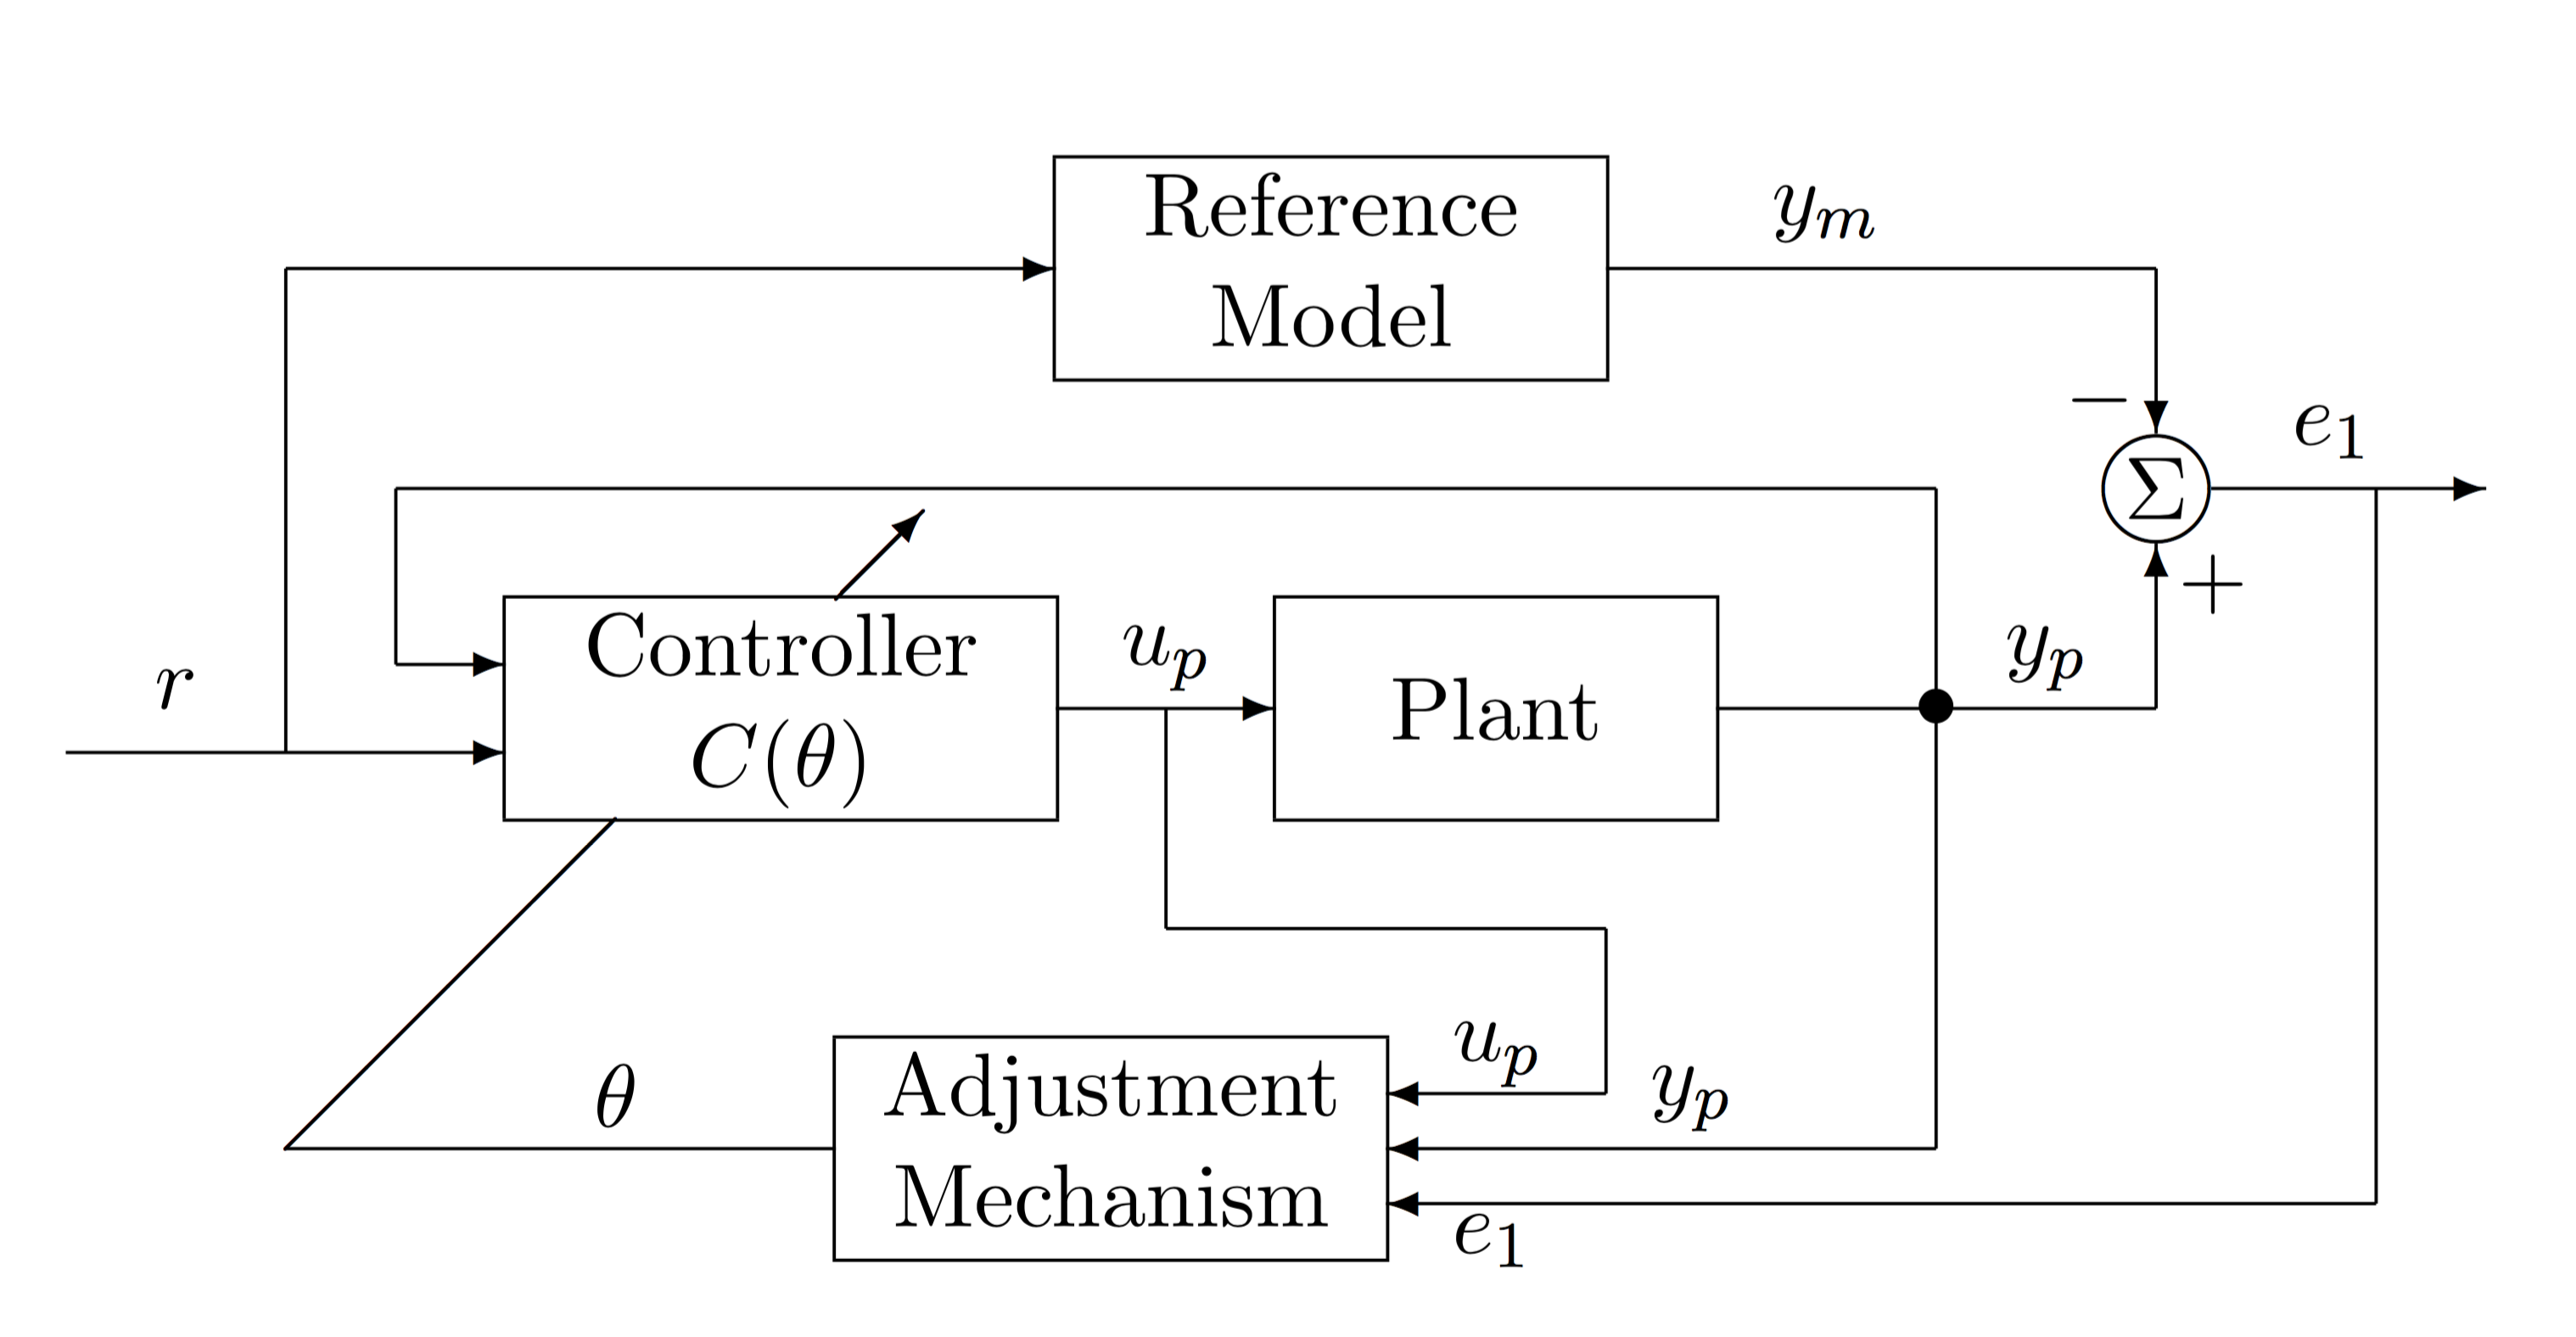
\includegraphics[width = \textwidth]{MRAC}
\caption{MRAC structure}
% \label{fig:MRAC}
\end{center}
\end{figure}

\subsection{How to... MRAC}
Given a plant $y(s) = \frac{b}{s+a}u(s)$ and a reference model $y_m(s) = \frac{b_m}{s+a_m}r$ where $r \in L_\infty$.
Then the optimal ideal controller has the structure $u^* = -\theta_1^* y + \theta_2^* r$, where $\theta_1^*$ and $\theta_2^*$ is optimal controller parameters. The optimal parameters can be found by comparison between $y$ and $y_m$:
\begin{equation}
\begin{split}
y &= \frac{b}{s+a}(-\theta_1^* y + \theta_2^* r) \\
y(1+\frac{b\theta_1^*}{s+a} ) &= \frac{b\theta_2^*}{s+a}r \\
y &= \frac{b\theta_2^*}{s+a+b\theta_1^*}r
\end{split}
\end{equation}
which gives us $\theta_1^* = \frac{a_m-a}{b}$ and $\theta_2^* = \frac{b_m}{b}$. The closed loop differential equations is

\begin{equation}
\begin{split}
\dot{y} &= -ay +bu \\
& =-ay + b (-\theta_1 y + \theta_2 r) \\
& = (-a- b \theta_1) y + b \theta_2 r \\
\dot{y_m} &= -a_m y_m + b_m r
\end{split}
\end{equation}
We now define $e \triangleq y - y_m$, $\tilde{\theta_1}  \triangleq \theta_1 - \theta_1^*$, $\tilde{\theta_2}  \triangleq \theta_2 - \theta_2^*$ and derive the error dynamics.

\begin{equation}
\begin{split}
\dot{e} &= \dot{y}-\dot{y_m} \\
&= (-a- b \theta_1) y + b \theta_2 r - ( -a_m y_m + b_m r ) \\
&= -a_m y +  a_m y_m + (-a + a_m- b \theta_1) y + b \theta_2 r - b_m r \\
&= -a_m e + (-a + a_m- b (\tilde{\theta_1} +\frac{a_m-a}{b})) y + b (\tilde{\theta_2} + \frac{b_m}{b})r - b_m r \\
&= -a_m e - \tilde{\theta_1}b y + \tilde{\theta_2}b r
\end{split}
\end{equation}
We now use a Lyapunov (ish?) function $V = \frac{1}{2}e^2 + \frac{b}{2\gamma_1}\tilde{\theta_1^2} + \frac{b}{2\gamma_2}\tilde{\theta_2^2} $.

\begin{equation}
\begin{split}
\dot{V} &= e\dot{e} 	+ \frac{b}{\gamma_1}\tilde{\theta_1}\dot{\tilde{\theta_1}}
				+ \frac{b}{\gamma_2} \tilde{\theta_2}\dot{\tilde{\theta_2}} \\
&= 	e (-a_m e - \tilde{\theta_1}b y + \tilde{\theta_2}b r)
	+ \frac{b}{\gamma_1}\tilde{\theta_1}\dot{\theta_1}
	+ \frac{b}{\gamma_2}\tilde{\theta_2}\dot{\theta_2} \\
&= -a_m e^2 	+ \frac{b}{\gamma_1}\tilde{\theta_1}(\dot{\theta_1}  - \gamma_1 y e)
			+ \frac{b}{\gamma_2}\tilde{\theta_2}(\dot{\theta_2} + \gamma_2 r e )
\end{split}
\end{equation}
The update laws are selected such that the derivative Lyapunov function are negative semi-definite.

\begin{equation}
\begin{split}
(\dot{\theta_1}  - \gamma_1 y e) &= 0 \Rightarrow \dot{\theta_1} = \gamma_1 y e \\
(\dot{\theta_2} + \gamma_2 r e ) &= 0 \Rightarrow \dot{\theta_2} = \gamma_2 r e
\end{split}
\end{equation}
It can now be shown that $e,\tilde{\theta_1}, \tilde{\theta_2},r,y_m,y,\dot{e} \in L_\infty$ and $e \in L_2$, which leads to $\lim_{t \to \infty} e(t) \rightarrow 0$ from Lemma 3.2.5.

%!TEX root = TTK4215-Summary.tex
\section{Adaptive pole placement control (APPC)}
APPC is pretty cool, because it does not require a plant of minimum phase (as opposed to MRAC).

\subsection{Indirect PPC}
Given the system
\begin{equation}
	y_p = \frac{Z_p(s)}{R_p(s)} u_p
\end{equation}
where
\begin{itemize}
	\item $R_p$ is monic, of known degree $n$,
	\item $Z_p, R_p$ are coprime,
	\item $G_p$ strictly proper ($\deg{Z_p} < n$).
\end{itemize}

The objective is to choose $u_p$ so that the closed-loop poles are the roots of a polynomial $A^*(s)$. Can be done by choosing $P$ (degree $q+n-1$) and $L$ (monic, degree $n-1$) such that
\begin{equation}
	L Q_m R_p + P Z_p = A^*
\end{equation}
is satisfied for $A^*$ of degree $2n+q-1$. $Q_m$ is chosen so that
\begin{equation}
	Q_m y_p = 0,
\end{equation}
and the control input is given by
\begin{equation}
	Q_m L u_p = -P (y_p - y_m)
	.
\end{equation}
%!TEX root = TTK4215-Summary.tex
\section{Robustness}

\subsection{Parameter drift}
An unknown bounded disturbance added to the measurement $y$ can lead to \emph{parameter drift}, meaning $\theta \to \infty$ as $t \to \infty$. The equilibrium $\tilde{\theta}_e = 0$ can be made u.a.s. by making $u(t)$ PE. (But we don't always decide $u(t)$.)

%!TEX root = TTK4215-Summary.tex
\section{Extremum seeking}
The basic idea: Want to find the optimal plant input $\theta^*$ that maximises the output $y$. Add a slow periodic perturbation to our estimate $\hat{\theta}$. If increasing $\theta$ increases $y$, then $y$ will oscillate in phase with $\theta$. In the opposite case, $y$ with be out of phase with $\theta$. The DC component of $y$ is removed with a high-pass filter, and the result multiplied with the perturbation signal. The product will have a positive DC component if $y$ and $\theta$ are in phase, and negative DC if they are out of phase. This DC component is extracted with a low-pass filter, and is then a value indicating how far off $\theta$ is, and in what direction. This is integrated and multiplied with a gain $k$ to form the estimate $\hat{\theta}$. Pretty clever.

\begin{figure}[htbp]
\begin{center}
	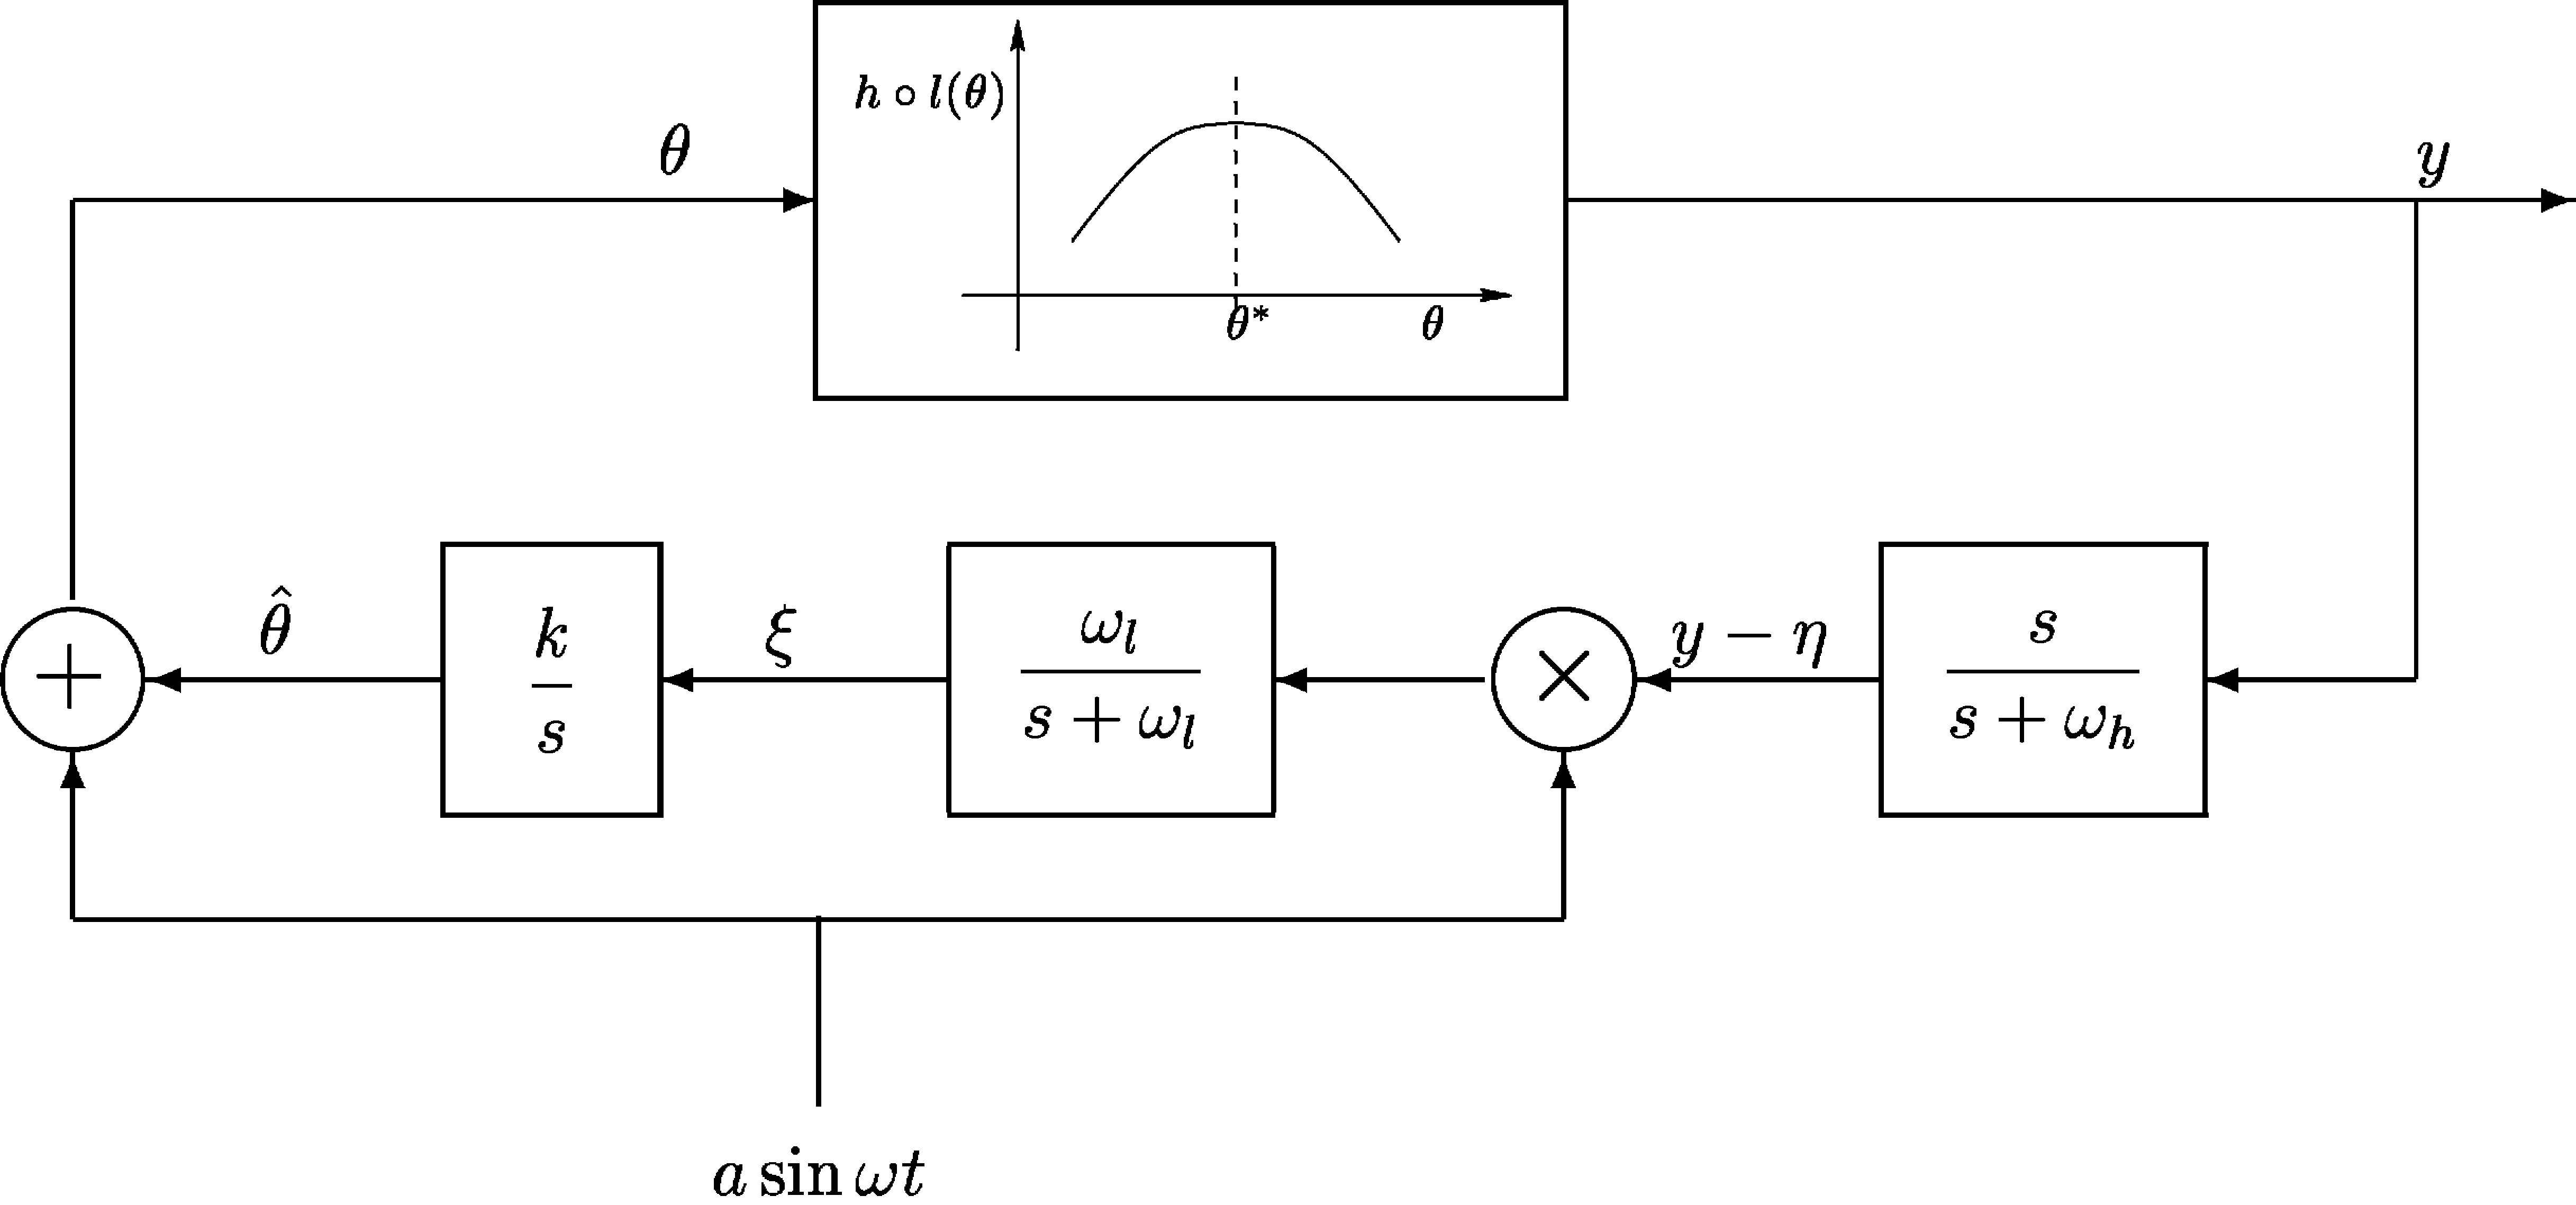
\includegraphics[width = \textwidth]{extremum-seeking}
	\caption{Block diagram for extremum seeking}
	\label{fig:MRAC}
\end{center}
\end{figure}

\end{document}